\documentclass[12pt,twoside]{article}
\usepackage{jmlda}
\usepackage[russian]{babel}
\long\def\comment{}
%\NOREVIEWERNOTES
\title
    [Декодирование сигналов мозга и прогнозирование намерений] % Краткое название; не нужно, если полное название влезает в~колонтитул
    {Декодирование сигналов мозга и прогнозирование намерений} % Краткое название; не нужно, если полное название влезает в~колонтитул
\author
    [Теленков~Д.\,С.] % список авторов для колонтитула; не нужен, если основной список влезает в колонтитул
    {Теленков~Д.\,С., Задаянчук~А.\,И., Стрижев~В.\,В.} % основной список авторов, выводимый в оглавление
    %[Стрижев~В.\,В.$^1$, Соавтор~И.\,О.$^2$, Фамилия~И.\,О.$^2$] % список авторов, выводимый в заголовок; не нужен, если он не отличается от основного

\email
    {telencov11@gmail.com}
\organization
    {$^1$Московский физико-технический институт; $^2$Сколковский институт науки и технологий}
\abstract
    {В данной статье исследуется проблема восстанавления движения конечностей по кортикограмме. Для решения задачи использовался алгоритм иерархической смеси экспертов над моделью PLS. Его результаты сравнивались с базовым алгоритмом Partial Least Squares. Сравнение показало, что алгоритм иерархической смеси экспертов над моделью PLS справляется с поставленной задачей лучше, что является следствием способа выбора признаков, учитывающего закономерности как в независимой, так и в зависимой переменной.

\bigskip
\textbf{Ключевые слова}: \emph {Partial Least Squares, Electrocorticography ,
еще ключевые слова}.}
\titleEng
    {JMLDA paper example: file jmlda-example.tex}
\authorEng
    {Author~F.\,S.$^1$, CoAuthor~F.\,S.$^2$, Name~F.\,S.$^2$}
\organizationEng
    {$^1$Organization; $^2$Organization}
\abstractEng
    {This document is an example of paper prepared with \LaTeXe\
    typesetting system and style file \texttt{jmlda.sty}.

    \bigskip
    \textbf{Keywords}: \emph{keyword, keyword, more keywords}.}
\begin{document}
\maketitle
%\linenumbers
\section{Введение}
Восстановление движений по сигналам мозга является важной задачей в наши дни. С ее помощью люди будут способны заменить потерянную конечность электронным протезом. Парализованные получат возможность говорить и передвигаться на автоматических колясках[5]. Кроме того, ее решения применимы в создании экзоскелетов.\par
Уже есть примеры успешных исследований в данной области. Используя метод электромиограммы, исследователи смогли вернуть способность к базовым движениям людям с латеральным склерозом и повреждениями спиного мозга [2, 3].  \par
Используемым нами методом снятия сигналов мозга является кортикограмма. Она получает данные из электродов, накладываемых непосредственно на кору головного мозга, под кости черепа. Исследования показывают, что кортикограмма является более точным и устойчивым методом, по сравнению с электромиограммой. Кортикограмма превосходит электромиограмму в амплитуде сигнала (обычно выше в пять раз), пространственном разрешении (0.125 против 3 см.) и полосе пропускания частот (0-550Гц. против 0-40Гц) [4].\par
Отличительной особенностью исследования является использование алгоритма понижения размерности, отличного от PLS. В схожей работе [4] исследователи из Вашингтонского университета добились высоких результатов в предсказывании движений пальцеав руки. Основными алгоритмами являлись PLS и логистическая регрессия. Для дальнейшего улучшения качества предсказания, нами предлагается использование алгоритма учитывающего неортогональную структуру взаимозависимости признаков для снижения размерности.\par
Для исследования базового алгоритма использовался датасет из работы [1]. В нем представлен временной ряд с показаниями кортикограммы в зависимости от напряжения пальцев руки.

\section{Постановка задачи}
Дана выборка размера $m$:
$$D_n = \{\pmb{x_i}, \pmb{y_i}\}^m_{i=1}$$
где $\pmb{x_i} \in \mathbb{R}^n$ - вектор признаков, $\pmb{y_i} \in \mathbb{R}^5$. Будем также говорить, что у нас есть матрица параметров $X$ и матрица ответов $Y$ \par
Выборка разбита на обучение и контроль:
$$D_\tau = \{\pmb{x_i}, \pmb{y_i}\}_{i\in\tau}\ \ D_\theta = \{\pmb{x_i}, \pmb{y_i}\}_{i\in\theta}\ \ \tau \sqcup \theta = [1, 2, \ldots, m]$$
Требуется научиться предсказывать значения $\pmb{y_i}$ по $\pmb{x_i}$ на обучении и проверить точность на контроле.

\paragraph{Базовый алгоритм}
В следствии высокой размерности и корреляции между компонентами $x_i$, проводится процедура понижения размерности. Для этого используется алгоритм partial least squares. Он находит переход из пространства параметров $\mathbb{R}^n$ в пространство более низкой размерности - $\mathbb{R}^k,\ k < n$, основываясь на корреляции между параметрами и ответами. Таким образом у нас появляются матрицы перехода - $W_{n \times k}$ и латентных переменных - $T_{m \times k} = X W$. Задача линейной регрессии переходит в нахождении $Q \in \mathbb{R}^k$, что:
$$Y = T Q + E = X W Q + E$$
$E$ - шум. Основная задача - нахождение $W$. \par
Существуют различные решения PLS. Остановимся на одном из самых популярных - NIPALS (nonlinear iterative partial least squares). Этот алгоритм итеративный. Каждая итерация занимает шесть шагов. Перед тем как их перечислить, следует ввести несколько обозначений: $A_1 = X^TY,\ M_1 = X^TX,\ C_1 = I$. На $i$-й итерации алгоритма происходит:
\begin{enumerate}
    \item вычислим $\pmb{e_i}$, доминантный собственный вектор $A_i^T A_i$
    \item $\pmb{w_i} = C_i A_i \pmb{e_i}, \pmb{w_i} = \frac{\pmb{w_i}}{||\pmb{w_i}||}$. Положим $\pmb{w_i}$ в $W$, как $i$-ю колону
    \item $\pmb{p_i} = M_i \pmb{w_i},\ c_i = \pmb{w_i}^T M_i \pmb{w_i},\ \pmb{p_i} = \frac{\pmb{p_i}}{c_i}$
    \item $\pmb{q_i} = \frac{A_i^T \pmb{w_i}}{c_i}$. Положим $\pmb{q_i}$ в $Q$, как $i$-ю колону
    \item $A_{i + 1} = A_i - c_i \pmb{p_i} \pmb{q_i}^T, M_{i + 1} = M_i - c_i \pmb{p_i} \pmb{p_i}^T$
    \item $C_{i + 1} = C_i - \pmb{w_i} \pmb{p_i}^T$
\end{enumerate}
 Чтобы перейти к размерности $k$ необходимо сделать $k$ итераций. На выходе мы получаем матрицы $W$ и $Q$, т.е. уже готовы к проверке на контрольной выборке.
 
 \section{Эксперимент}
 Для сравнения базового и основного алгоритмов использовался один и тот же датасет, взятый из работы [1]. В нем показаниям с 64 каналов кортикограммы сопоставлялись натяжения во всех пяти пальцах руки испытуемой. Частота сэмплирования - 1кГц, полоса пропускания каналов - 0.15-200Гц.
 
 \paragraph{Датасет}
 Датасет состоит из элементов:
$$D_n = \{\pmb{x_i}, \pmb{y_i}\}^{4\cdot10^6}_{i=1},$$
где $\pmb{x_i} \in \mathbb{R}^{64}$ - вектор признаков, $\pmb{y_i} \in \mathbb{R}^5$.

\paragraph{Базовый алгоритм}
Для проверки качества базового алгоритма использовалась кросс-валидация. Гиперпараметр размерности нового пространства параметров варьировался от 1 до 64. Посмотрим на результаты:  
\begin{figure}[h]
    \begin{minipage}[h]{1\linewidth}
    \center{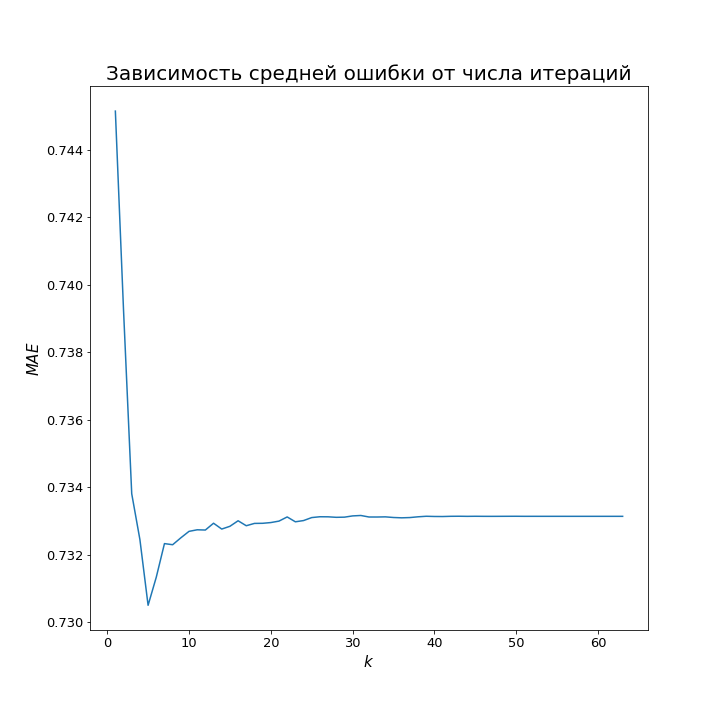
\includegraphics[width=1\textwidth]{error.eps}} 
    \center{\caption{Зависимость средней ошибки от числа итераций.}}
    \end{minipage}
\label{fg:Example}
\end{figure}
\par
Как и предполагалось, есть минимум функционала ошибки, в следствии зависимости в параметрах. Занимательным является тот факт, что наилучшая итоговая размерность совпадает с размерностью пространства откликов. Минимальное MAE - 0.731.

\section{Литература}
[1] Schalk, G., Kubanek, J., Miller, K.J., Anderson, N.R., Leuthardt, E.C., Ojemann, J.G., Limbrick, D., Moran, D.W., Gerhardt, L.A., and Wolpaw, J.R. Decoding TwoDimensional Movement Trajectories Using Electrocorticographic Signals in Humans, J Neural Eng, 4: 264-275, 2007. \par
[2] Decoding Ipsilateral Finger Movements from ECoG Signals in Humans \par
[3] J. Wolpaw, N. Birbaumer, D. McFarland, G. Pfurtscheller, and T. Vaughan. Brain-computer interfaces for communication and control. Clinical neurophysiology, 113(6):767–791, 2002. \par 
[4] G. Pfurtscheller, C. Guger, G. Muller, G. Krausz, and C. Neuper. Brain oscillations control hand orthosis in a tetraplegic. Neuroscience letters, 292(3):211–214, 2000. \par
[5] J. Wolpaw and D. McFarland. Control of a two-dimensional movement signal by a noninvasive brain-computer interface in humans. Proceedings of the National Academy of Sciences of the United States of America, 101(51):17849, 2004.

\bibliographystyle{unsrt}
\bibliography{jmlda-bib}
%\begin{thebibliography}{1}

%\bibitem{author09anyscience}
%    \BibAuthor{Author\;N.}
%    \BibTitle{Paper title}~//
%    \BibJournal{10-th Int'l. Conf. on Anyscience}, 2009.  Vol.\,11, No.\,1.  Pp.\,111--122.
%\bibitem{myHandbook}
%    \BibAuthor{Автор\;И.\,О.}
%    Название книги.
%    Город: Издательство, 2009. 314~с.
%\bibitem{author09first-word-of-the-title}
%    \BibAuthor{Автор\;И.\,О.}
%    \BibTitle{Название статьи}~//
%    \BibJournal{Название конференции или сборника},
%    Город:~Изд-во, 2009.  С.\,5--6.
%\bibitem{author-and-co2007}
%    \BibAuthor{Автор\;И.\,О., Соавтор\;И.\,О.}
%    \BibTitle{Название статьи}~//
%    \BibJournal{Название журнала}. 2007. Т.\,38, \No\,5. С.\,54--62.
%\bibitem{bibUsefulUrl}
%    \BibUrl{www.site.ru}~---
%    Название сайта.  2007.
%\bibitem{voron06latex}
%    \BibAuthor{Воронцов~К.\,В.}
%    \LaTeXe\ в~примерах.
%    2006.
%    \BibUrl{http://www.ccas.ru/voron/latex.html}.
%\bibitem{Lvovsky03}
%    \BibAuthor{Львовский~С.\,М.} Набор и вёрстка в пакете~\LaTeX.
%    3-е издание.
%    Москва:~МЦHМО, 2003.  448~с.
%\end{thebibliography}

% Решение Программного Комитета:
%\ACCEPTNOTE
%\AMENDNOTE
%\REJECTNOTE
\end{document}